%% This is an example first chapter.  You should put chapter/appendix that you
%% write into a separate file, and add a line \include{yourfilename} to
%% main.tex, where `yourfilename.tex' is the name of the chapter/appendix file.
%% You can process specific files by typing their names in at the 
%% \files=
%% prompt when you run the file main.tex through LaTeX.
\chapter{Surveys, simulation, and single-cell assays relate function and phylogeny in a lake ecosystem}
\label{ch:lake}

The contents of this chapter were accepted as: 
Sarah P. Preheim$^*$, Scott W. Olesen$^*$ (these authors contributed equally), Sarah J. Spencer, Arne Materna,
Charuleka Varadharajan, Matthew Blackburn, Jonathan Friedman, Jorge
Rodr\'{i}guez, Harold Hemond and Eric J. Alm.
(2016) \textit{Nature Microbiology}.

The figures are at the end of the chapter. The Supplementary Information is in Appendix A.

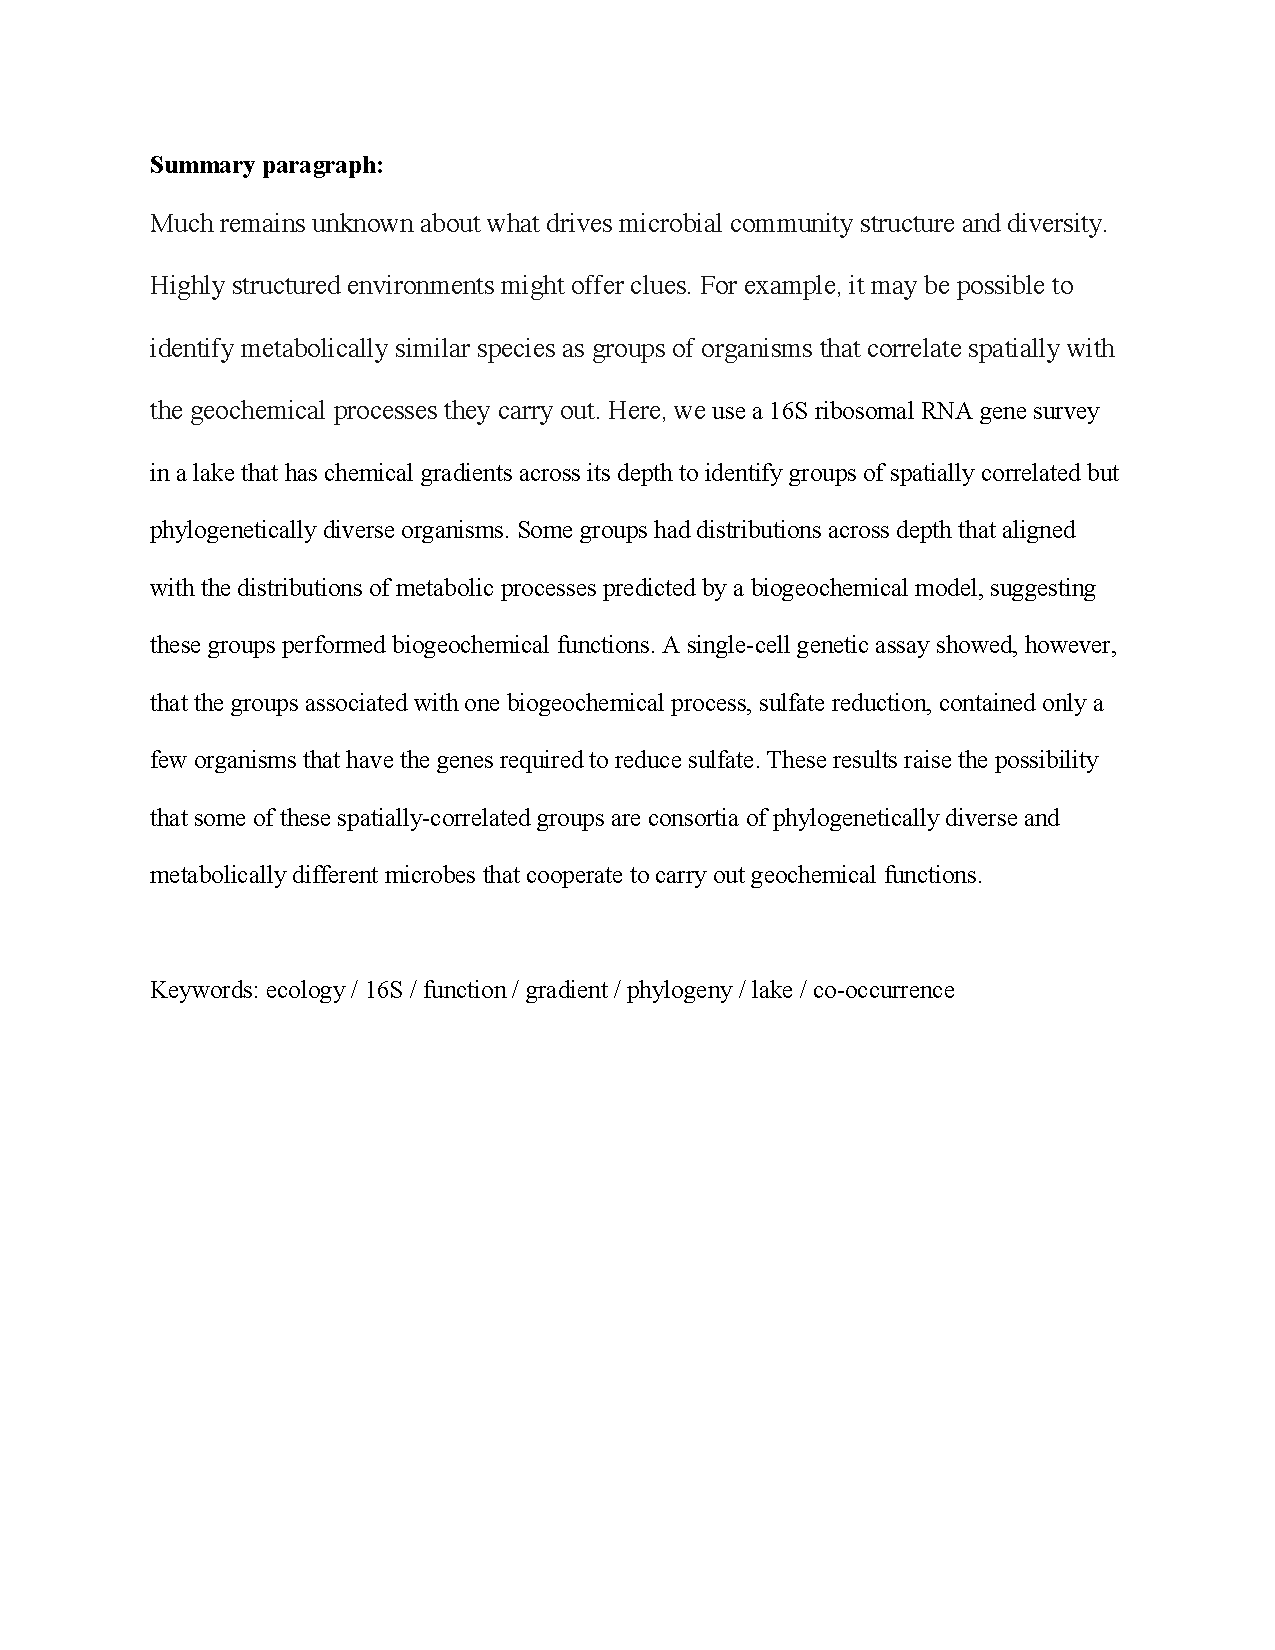
\includepdf[pages=-, pagecommand={\thispagestyle{plain}}]{lake/ms}

\begin{figure}[ht]
\centering
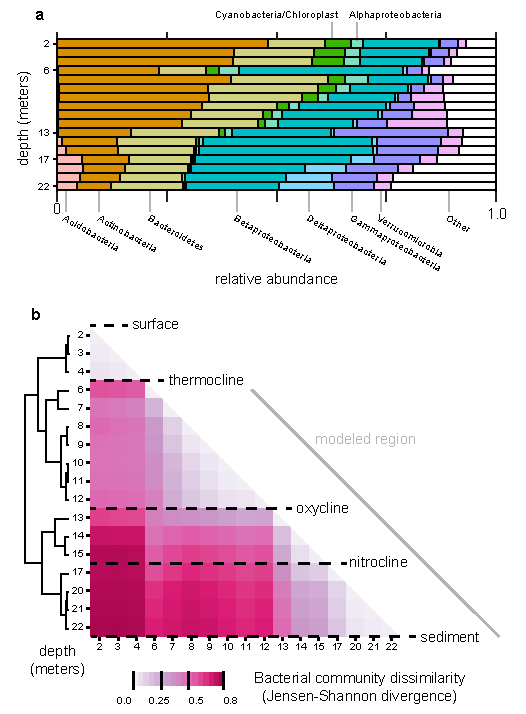
\includegraphics{lake/fig/fig1}
\caption*{{\bf Figure 1.} Bacterial survey of the lake identified communities
that vary with depth. {\bf a} The relative abundance of the seven most abundant phyla
at four representative depths. Proteobacteria is divided into the classes $\alpha$-,
$\beta$-, $\gamma$-, and $\delta$-Proteobacteria. ($\varepsilon$-Proteobacteria were 
not abundant [$< 0.5\%$ at
every depth] and are not shown.) {\bf b} Each square shows the dissimilarity between
bacterial communities at two depths (e.g., the lower-left square shows the
dissimilarity between the samples from the surface and from 22 meters depth).
Major features (dotted lines) of the lake are noted: the thermocline, where the
temperature gradient is steepest; the oxycline, where dissolved oxygen falls to
0.3 mg/L; the nitrocline, where nitrate concentration falls below detection;
and the sediment at the lake bottom. The biogeochemical model treats the region
below the thermocline (gray line).}
\end{figure}

\begin{figure}[ht]
\centering
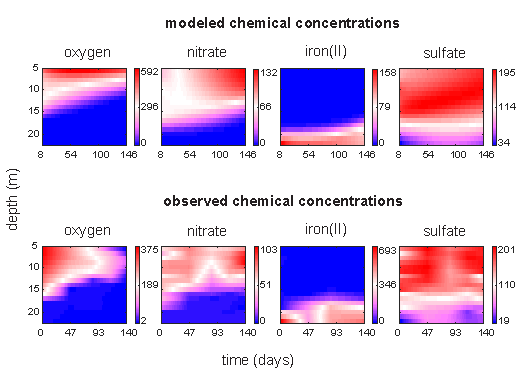
\includegraphics{lake/fig/fig2}
\caption*{{\bf Figure 2.} The model creates a dynamic picture of chemical
changes that occur in the lake through the lake's depth (vertical axis) across
time (horizontal). The model predicts changes in chemical species (top row;
colorbar scales are $\mu$M) which are consistent with the observed chemical
dynamics within the lake in 2013 (bottom row; colorbar scales are $\mu$M;
interpolated from five timepoints for oxygen, nitrate and sulfate and
interpolated from four time points for iron). The model was initiated from the
observed conditions in March 2013. Only a subset of chemical species included
in the model are shown.}
\end{figure}

\begin{figure}[ht]
\centering
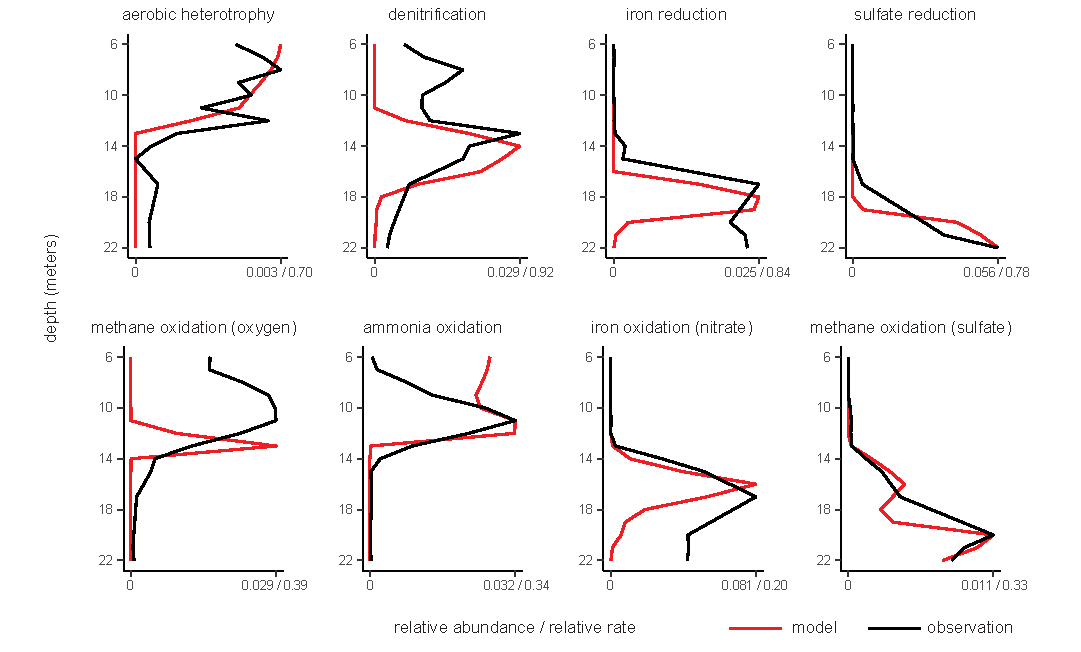
\includegraphics[width=\textwidth]{lake/fig/fig3}
\caption*{{\bf Figure 3.} Distribution of key populations (black lines,
relative abundance) from 2013 and their correspondence with modeled processes
(red lines, relative rate). Even though the two sets of lines represent
entirely different quantities (relative abundance of an organism vs. relative
prevalence of a metabolic process) their peaks and sometimes their spreads
roughly correspond, suggesting that the distribution of these organisms is
largely determined by the relative favorability of the modeled metabolic
processes within the lake.}
\end{figure}

\begin{figure}[ht]
\centering
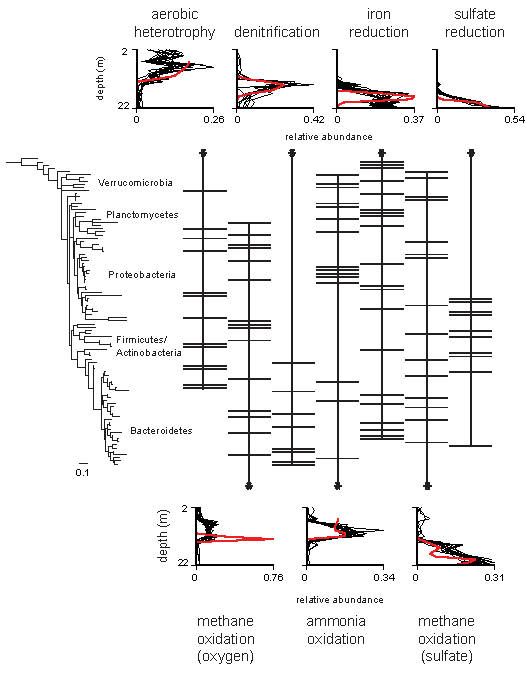
\includegraphics{lake/fig/fig4}
\caption*{{\bf Figure 4.} Operational ecological units (OEUs) are comprised of
phylogenetically diverse OTUs that largely align with modeled processes. The
phylogenetic tree (left; scale bar is substitutions per site) shows the
relationship between OTUs' representative 16S rRNA gene sequences in OEUs
containing key populations. Every OTU (on the rows) in the tree is a member of
one OEU (on the columns). Each bar indicates that the OTU in that row belongs
to the OEU represented by that column. Each inset shows the distributions
(black lines) with depth for OTUs in that OEU as well as the distribution (red
line) of a biogeochemical process (inset labels) predicted by the model. The
insets above and below the main figure correspond to the adjacent OEU columns
marked by asterisks. Modeled processes are only shown for the modeled region,
i.e., below 5 meters depth. OEUs were matched to the modeled processes as
described in the Methods.}
\end{figure}

\begin{figure}[ht]
\centering
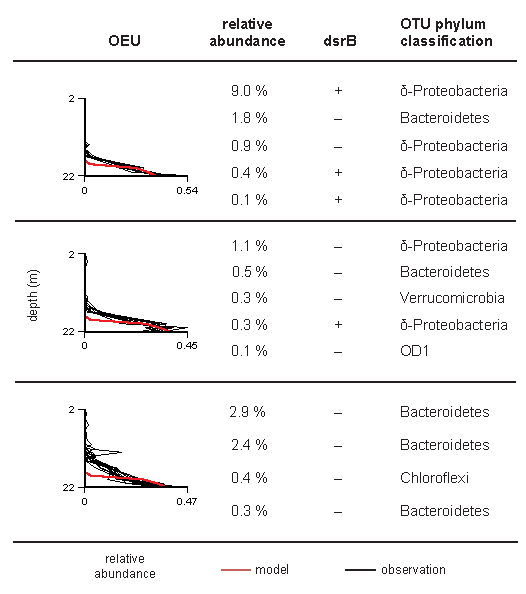
\includegraphics{lake/fig/fig5}
\caption*{{\bf Figure 5.} OEUs corresponding to sulfate reduction do not have
metabolically identical OTUs. The three OEUs with profiles corresponding to
sulfate reduction in the model are shown (the black lines are OTUs within each
OEU; the red lines are the relative rate of sulfate reduction predicted by the
model). The rows in each OEU correspond to each of that OEU's member OTUs. Of
these three OEUs, the single-cell assay determined that two OEUs contained
member OTUs that carry the diagnostic enzyme for sulfate reduction. The
relative abundance in the second column is percent of the control non-specific
16S-barcode fusion library corresponding to each OTU sequence. The third column
indicates whether a fusion product was identified in the \textit{dsrB}-16S gene fusion
library ($+$/$-$). The fourth column indicates phylum level classification for each
OTU, even if the OTU could be classified at a lower taxonomic rank.}
\end{figure}
